\documentclass{article}

\usepackage[a4paper, total={6.5in, 9.6in}]{geometry}
\usepackage{courier}
\usepackage{listings}
\usepackage{xcolor}
\usepackage{hyperref}
\usepackage{amsmath}
\usepackage{graphicx}
\usepackage{fontspec}
\setmainfont{Ubuntu}
%\setsansfont{Ubuntu}
\setmonofont{JetBrainsMono Nerd Font Mono}
% \setmonofont{}

\definecolor{mygreen}{rgb}{0.05,0.15,0.11}
\definecolor{mygray}{rgb}{0.5,0.5,0.5}
\definecolor{mymauve}{rgb}{0.58,0,0.82}

\lstset{
  backgroundcolor=\color{white}, basicstyle=\ttfamily, breakatwhitespace=false,
  breaklines=true, commentstyle=\color{darkgray}, keepspaces=true,
  keywordstyle=\bfseries\color{black}, morekeywords={*,...},
  showspaces=false, showstringspaces=false, showtabs=false, 
  stringstyle=\color{blue}, tabsize=4,
}

\begin{document}

\pagenumbering{gobble}
\newpage
\section*{Question 1}
Design a LEX Code to count the number of lines, space,
tab-meta character, and rest of characters in each Input
pattern.
\subsection*{Code:}
\lstinputlisting[language=C]{1/prog.l}
\newpage
\subsection*{Output:}
% \lstinputlisting{1/out.txt}
\begin{center}
  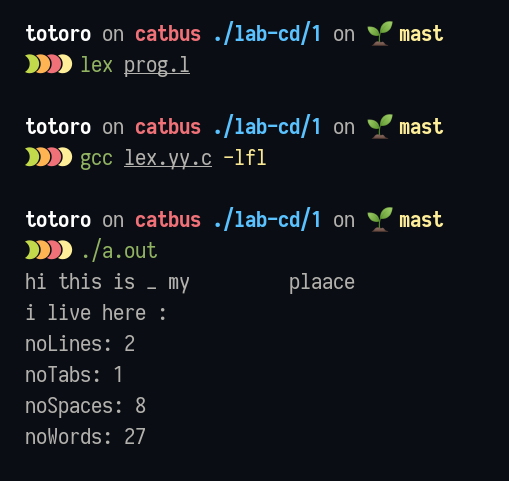
\includegraphics[width=9cm]{1/out.png}
\end{center}

\newpage
\section*{Question 2}
Design a LEX Code to identify and print valid Identifier of
C/C++ in given Input pattern.
\subsection*{Code:}
\lstinputlisting[language=C]{2/prog.l}
\newpage
\subsection*{Output:}
% \lstinputlisting{2/out.txt}
\begin{center}
  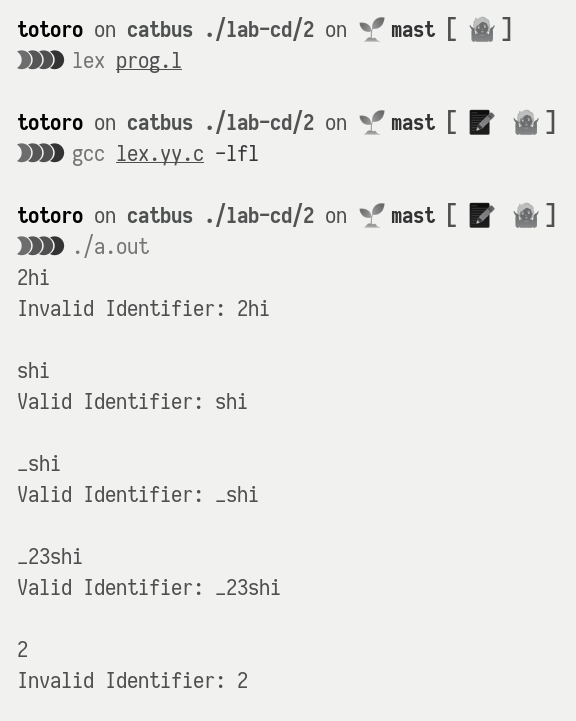
\includegraphics[width=9cm]{2/out.png}
\end{center}

\newpage
\section*{Question 3}
Design a LEX Code to identify and print integer and float
value in given Input pattern.
\subsection*{Code:}
\lstinputlisting[language=C]{3/prog.l}
\newpage
\subsection*{Output:}
% \lstinputlisting{3/out.txt}
\begin{center}
  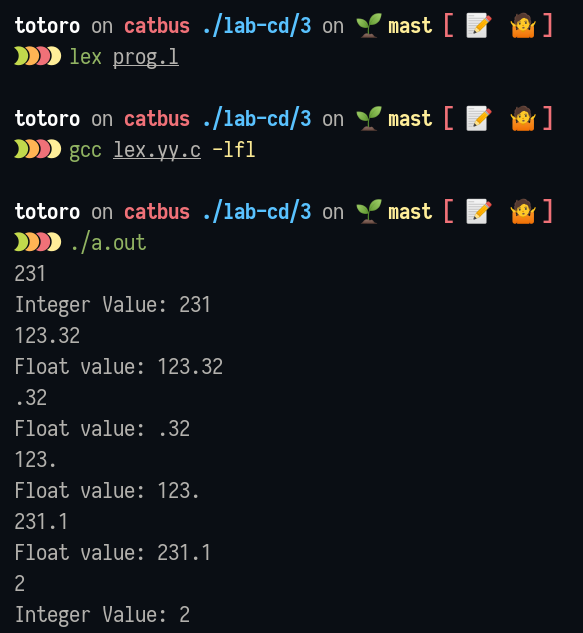
\includegraphics[width=10cm]{3/out.png}
\end{center}

\newpage
\section*{Question 4}
Design a LEX Code for Tokenizing
(Identify and print OPERATORS, SEPARATORS, KEYWORDS,
IDENTIFIERS)  from `in.c' file.
\subsection*{Code:}
\lstinputlisting[language=C]{4/prog.l}
\newpage
\subsection*{Output:}
\subsubsection*{Input File:}
\lstinputlisting{4/in.c}
\subsubsection*{Output File:}
\lstinputlisting{4/out.txt}

\newpage
\section*{Question 5}
Design a LEX Code to count and print the number of total
characters, words, white spaces in given Input.txt file.
\subsection*{Code:}
\lstinputlisting[language=C]{5/prog.l}
\newpage
\subsection*{Output:}
\subsubsection*{Input File:}
\lstinputlisting{5/input.txt}
\subsubsection*{Output:}
\lstinputlisting{5/output.txt}

\newpage
\section*{Question 6}
Design a LEX Code to replace white spaces of Input.txt
file by a single blank character into Output.txt file.
\subsection*{Code:}
\lstinputlisting[language=C]{6/prog.l}
\newpage
\subsection*{Output:}
\subsubsection*{Input File:}
\lstinputlisting{6/input.txt}
\subsubsection*{Output File:}
\lstinputlisting{6/output.txt}

\newpage
\section*{Question 7}
Design a LEX Code to remove the comments from any C-Program
given at run-time and store into out.c file.
\subsection*{Code:}
\lstinputlisting[language=C]{7/prog.l}
\newpage
\subsection*{Output:}
\subsubsection*{Input File:}
\lstinputlisting{7/input.c}
\subsubsection*{Output File:}
\lstinputlisting{7/out.c}

\newpage
\section*{Question 8}
Design a LEX Code to extract all html tags in the given HTML file
at run time and store into Text file given at run time.
\subsection*{Code:}
\lstinputlisting[language=C]{8/prog.l}
\newpage
\subsection*{Output:}
\subsubsection*{Input File:}
\lstinputlisting{8/ihtml.html}
\subsubsection*{Output File:}
\lstinputlisting{8/out.html}

\newpage
\section*{Question 9}
Design a DFA in LEX Code which accepts string containing even 
number of 'a' and even number of 'b' over input alphabet {a, b}.
\subsection*{Code:}
\lstinputlisting[language=C]{9/prog.l}
\newpage
\subsection*{Output:}
\begin{center}
  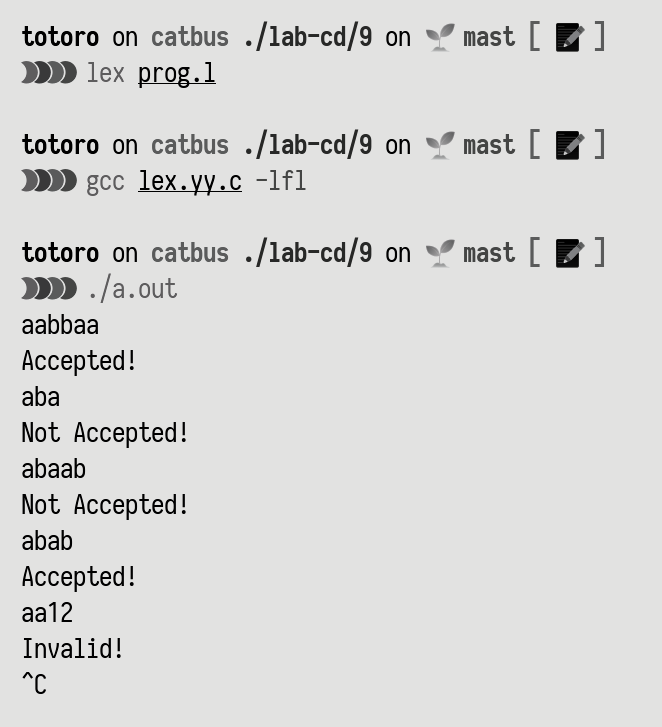
\includegraphics[width=9cm]{9/out.png}
\end{center}

\newpage
\section*{Question 10}
Design a DFA in LEX Code which accepts string containing third 
last element 'a' over input alphabet {a, b}.
\subsection*{Code:}
\lstinputlisting[language=C]{10/prog.l}
\newpage
\subsection*{Output:}
\begin{center}
  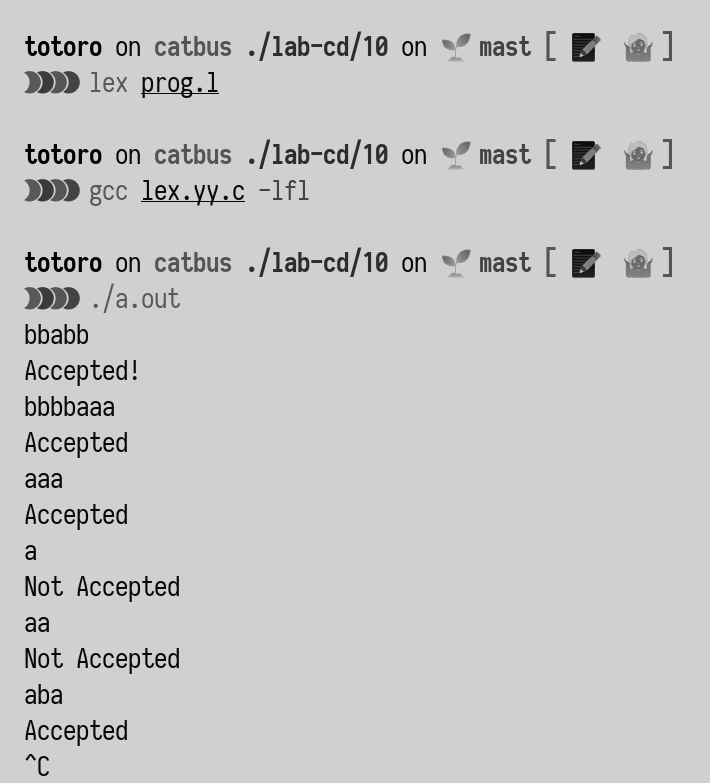
\includegraphics[width=9cm]{10/out.png}
\end{center}

\newpage
\section*{Question 11}
Design a DFA in LEX Code to Identify and print Integer and Float Constants and Identifier.
\subsection*{Code:}
\lstinputlisting[language=C]{11/prog.l}
\newpage
\subsection*{Output:}
\begin{center}
  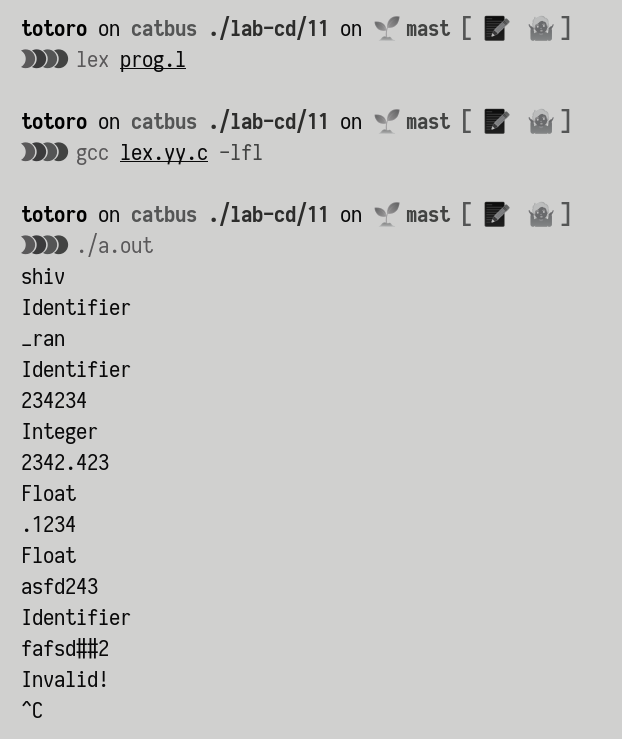
\includegraphics[width=9cm]{11/out.png}
\end{center}


\end{document}